Desde su nacimiento en 2013 hasta su expansión mundial hace poco más de 4 años, en
2017/18, los contenedores se han convertido en el \textit{modus operandi}
de muchas empresas, que han visto en la tecnología de contenedores una gran ventaja
y forma de despegar y aumentar su producción.

Desde entonces, diversos estudios como el llevado a cabo por Portworx cada año brindan
la oportunidad de ver qué tecnologías dominan el mercado y cómo va evolucionando el
mundo de los contenedores.

De entre los datos obtenidos, es destacable la adopción de contenedores en las
empresas tecnológicas: un 87\% de los encuestados (2019) afirman usar contenedores en
comparación con el 55\% registrado en 2017. Es más, el 90\% de las aplicaciones que
ejecutan en esos contenedores están en entornos de producción, una gran diferencia con
2018 (84\%) y 2017 (67\%) \cite{wattsStateContainersToday}.

Estos datos radican en la inversión económica que las empresas realizan en labores
de ``contenerización'', invirtiendo entre $\$\numprint{500000}$ y $\$\numprint{1000000}$
\cite{wattsStateContainersToday}. De entre todos los motivos que mueven a las empresas
a realizar esas inversiones, prima la seguridad de los datos sobre los demás.

Parece ser que una de las principales labores de los contenedores en estas decisiones
es la de proteger la información (61\%), gestionar las vulnerabilidades fácilmente
(43\%) y proteger el sistema en tiempo de ejecución (34\%). Estos datos van directamente
ligados con las medidas de seguridad que las compañías adoptan al usar contenedores:

\begin{itemize}
    \item Cifrar los datos (64\%).
    \item Monitorización en tiempo de ejecución (49\%).
    \item Escaneo de vulnerabilidades en los registros de contenedores (49\%).
    \item Escaneo de vulnerabilidades en las operaciones de CI/CD (49\%).
    \item Bloquear anomalías mediante la protección en tiempo de ejecución (48\%).
\end{itemize}

El siguiente motivo de la gran adopción de contenedores es que agiliza mucho la
velocidad en el desarrollo y la eficiencia. Por otra parte, la portabilidad de los
contenedores permite a las empresas poder mover sus entornos de producción y
desarrollo entre una y otra plataforma de nube públicas, de entre las cuales las
más usadas (12\% de la muestra) son AWS, Azure y Google Cloud \cite{wattsStateContainersToday}.

En particular, se observa cómo AWS (la plataforma de Amazon) es la dominante en este
sector, llevándose el 78\% del sector; la siguiente, Azure con el 39\%; y finalmente,
GCP (\textit{Google Cloud Platform}) con el 35\% y subiendo rápidamente \cite{ContainerAdoptionTrends}.
Destaca el crecimiento de Google ya que es quien empezó a invertir mucho dinero en
contenedores desde su nacimiento y el creador de Kubernetes, la tecnología de
orquestación más usada a nivel mundial.

\begin{figure}[H]
    \centering
    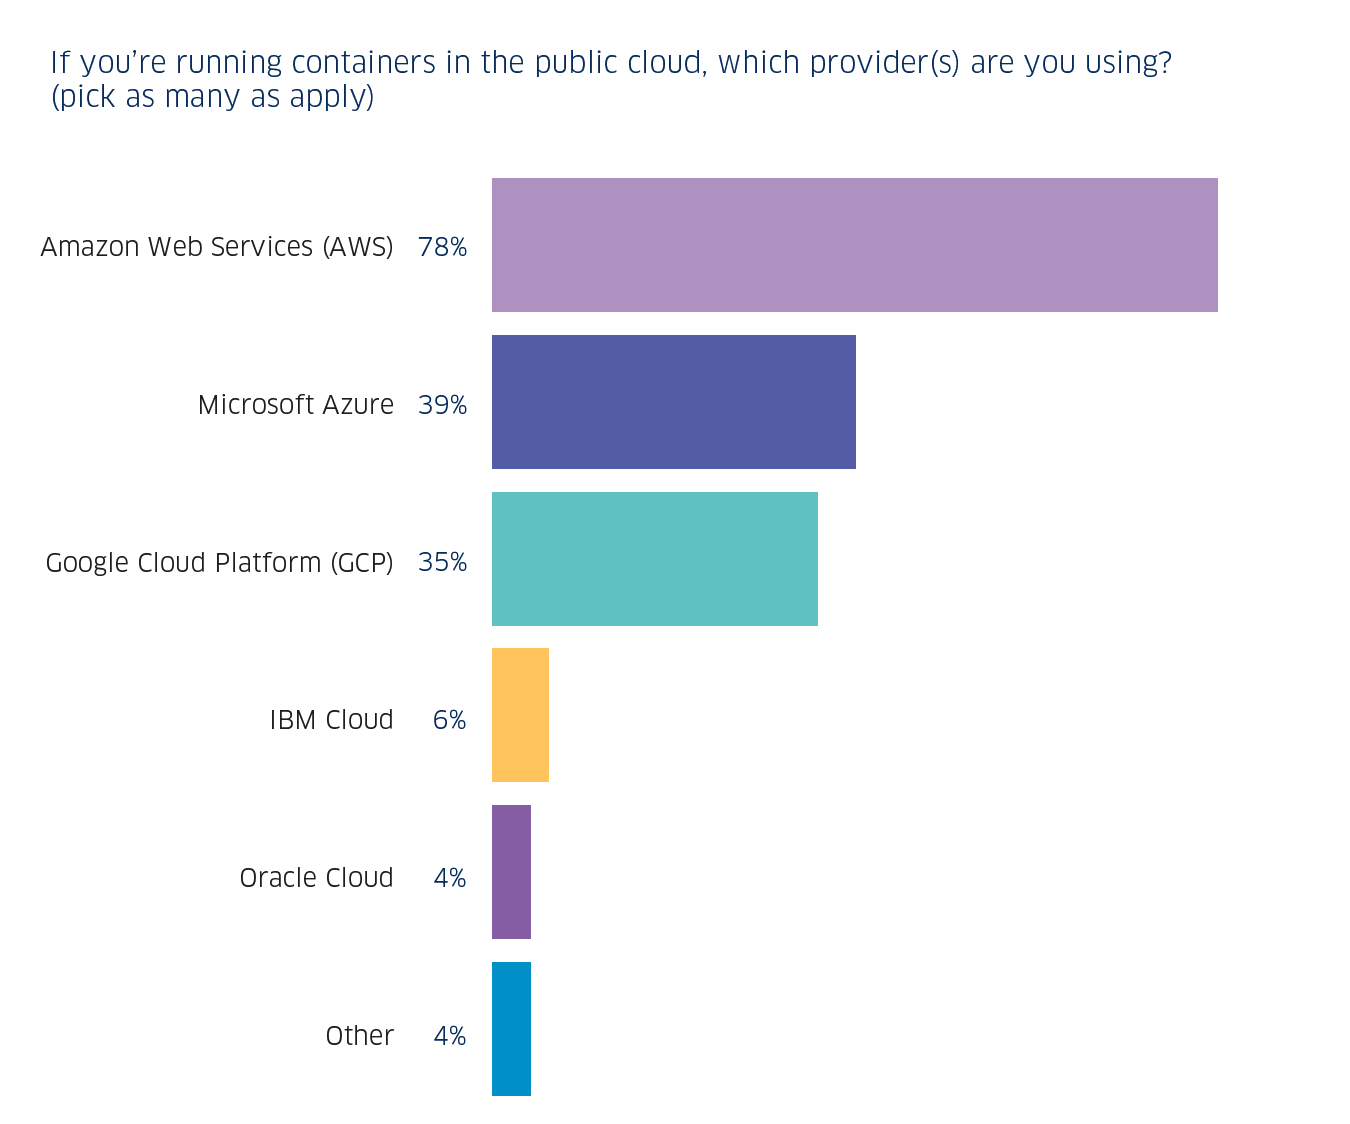
\includegraphics[width=.5\linewidth]{pictures/containers-in-the-cloud.png}
    \caption{Uso de contenedores según la plataforma \textit{cloud} \cite{ContainerAdoptionTrends}.}
\end{figure}

La situación mencionada anteriormente se ve directamente reflejada en la ``contenerización''
de aplicaciones en según que plataforma. De los usuarios de Azure, solo el 20\% ha
creado un contenedor para más de la mitad de sus aplicaciones, significativamente
más bajo que el 33\% de los no usuarios. Esto se ve drásticamente reducido cuando
se hablan de aplicaciones en entorno de producción \cite{ContainerAdoptionTrends}.

Por el contrario, casi un tercio de los usuarios de GCP (31\%) han creado un contenedor
para más de la mitad de sus aplicaciones, relativamente superior al 27\% de los
no usuarios. Este mismo efecto se produce con respecto a las aplicaciones en
producción desplegadas en GCP \cite{ContainerAdoptionTrends}.

Esto se ve reflejado en el gráfico de la figura \ref{fig:contenerized-apps}:

\begin{figure}[H]
    \centering
    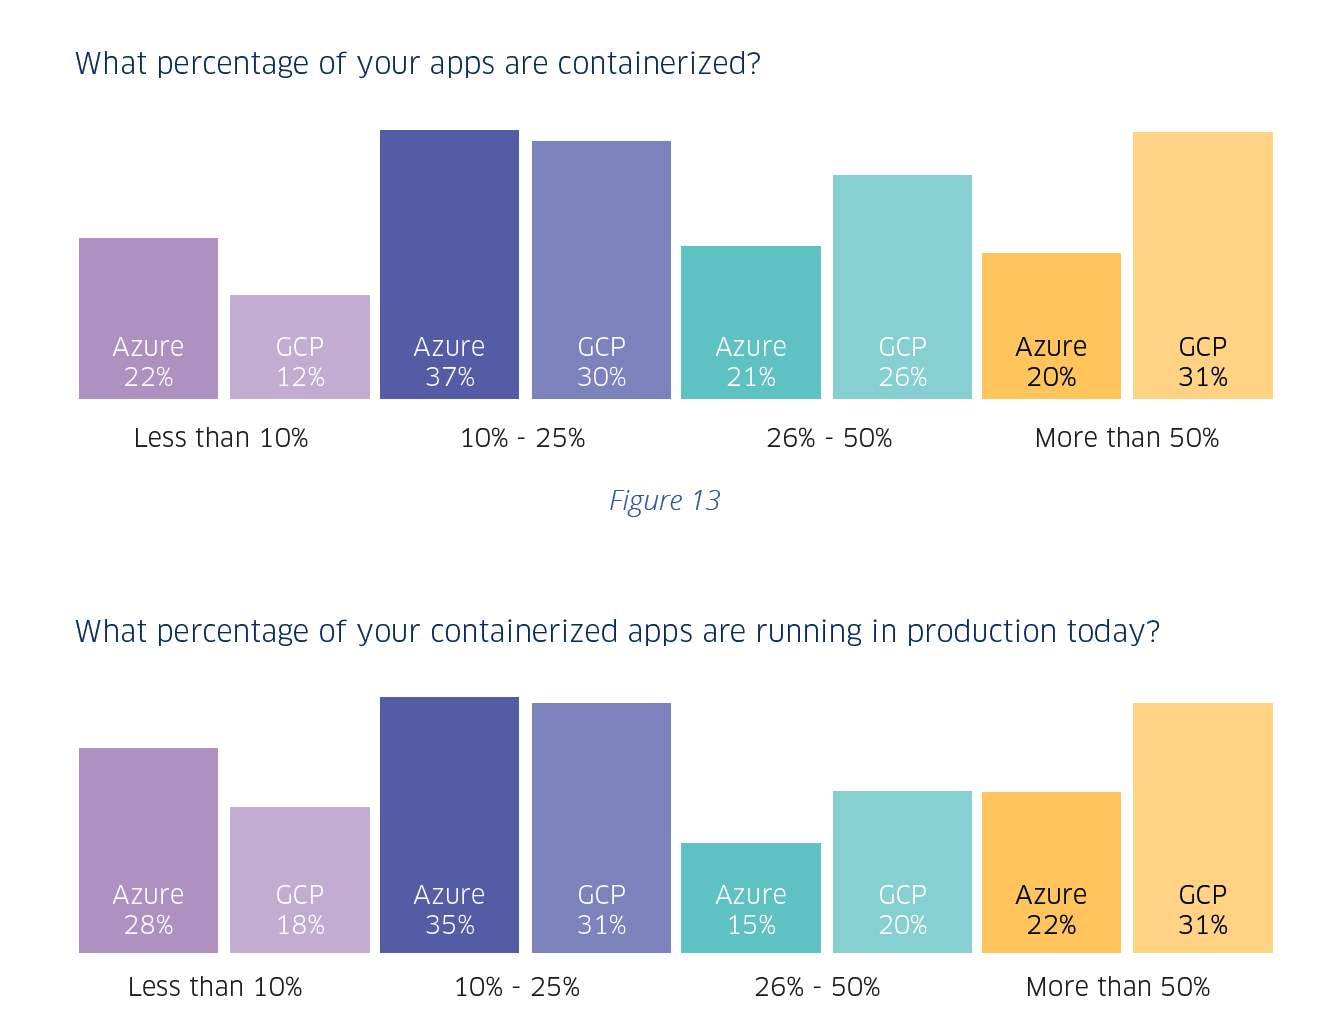
\includegraphics[width=.5\linewidth]{pictures/gcp-vs-azure.png}
    \caption{Porcentaje de las aplicaciones desplegadas en contenedores en según qué plataformas \cite{ContainerAdoptionTrends}.}
    \label{fig:contenerized-apps}
\end{figure}

En un estudio más moderno, se estima en el año 2020 ha supuesto un mayor auge en 
las tecnologías de ``contenerización'', en donde los responsables de IT han priorizado
la creación de contenedores para aplicaciones ya existentes, migrar toda la infraestructura
a la nube y hacer un mejor uso de las plataformas en la nube. De entre todos los
problemas, el principal es cumplir con los requisitos legales, de rendimiento y 
regulatorios vigentes según las necesidades de la industria; y la portabilidad
de las aplicaciones, las cuales estaban confinadas y diseñadas para sistemas en
particular y ahora se quieren desplegar en la nube en general \cite{ContainerAdoptionStatistics}.

Esto se ve en la infografía diseñada por Forrester (figura \ref{fig:container-stats}):

\begin{figure}[H]
    \centering
    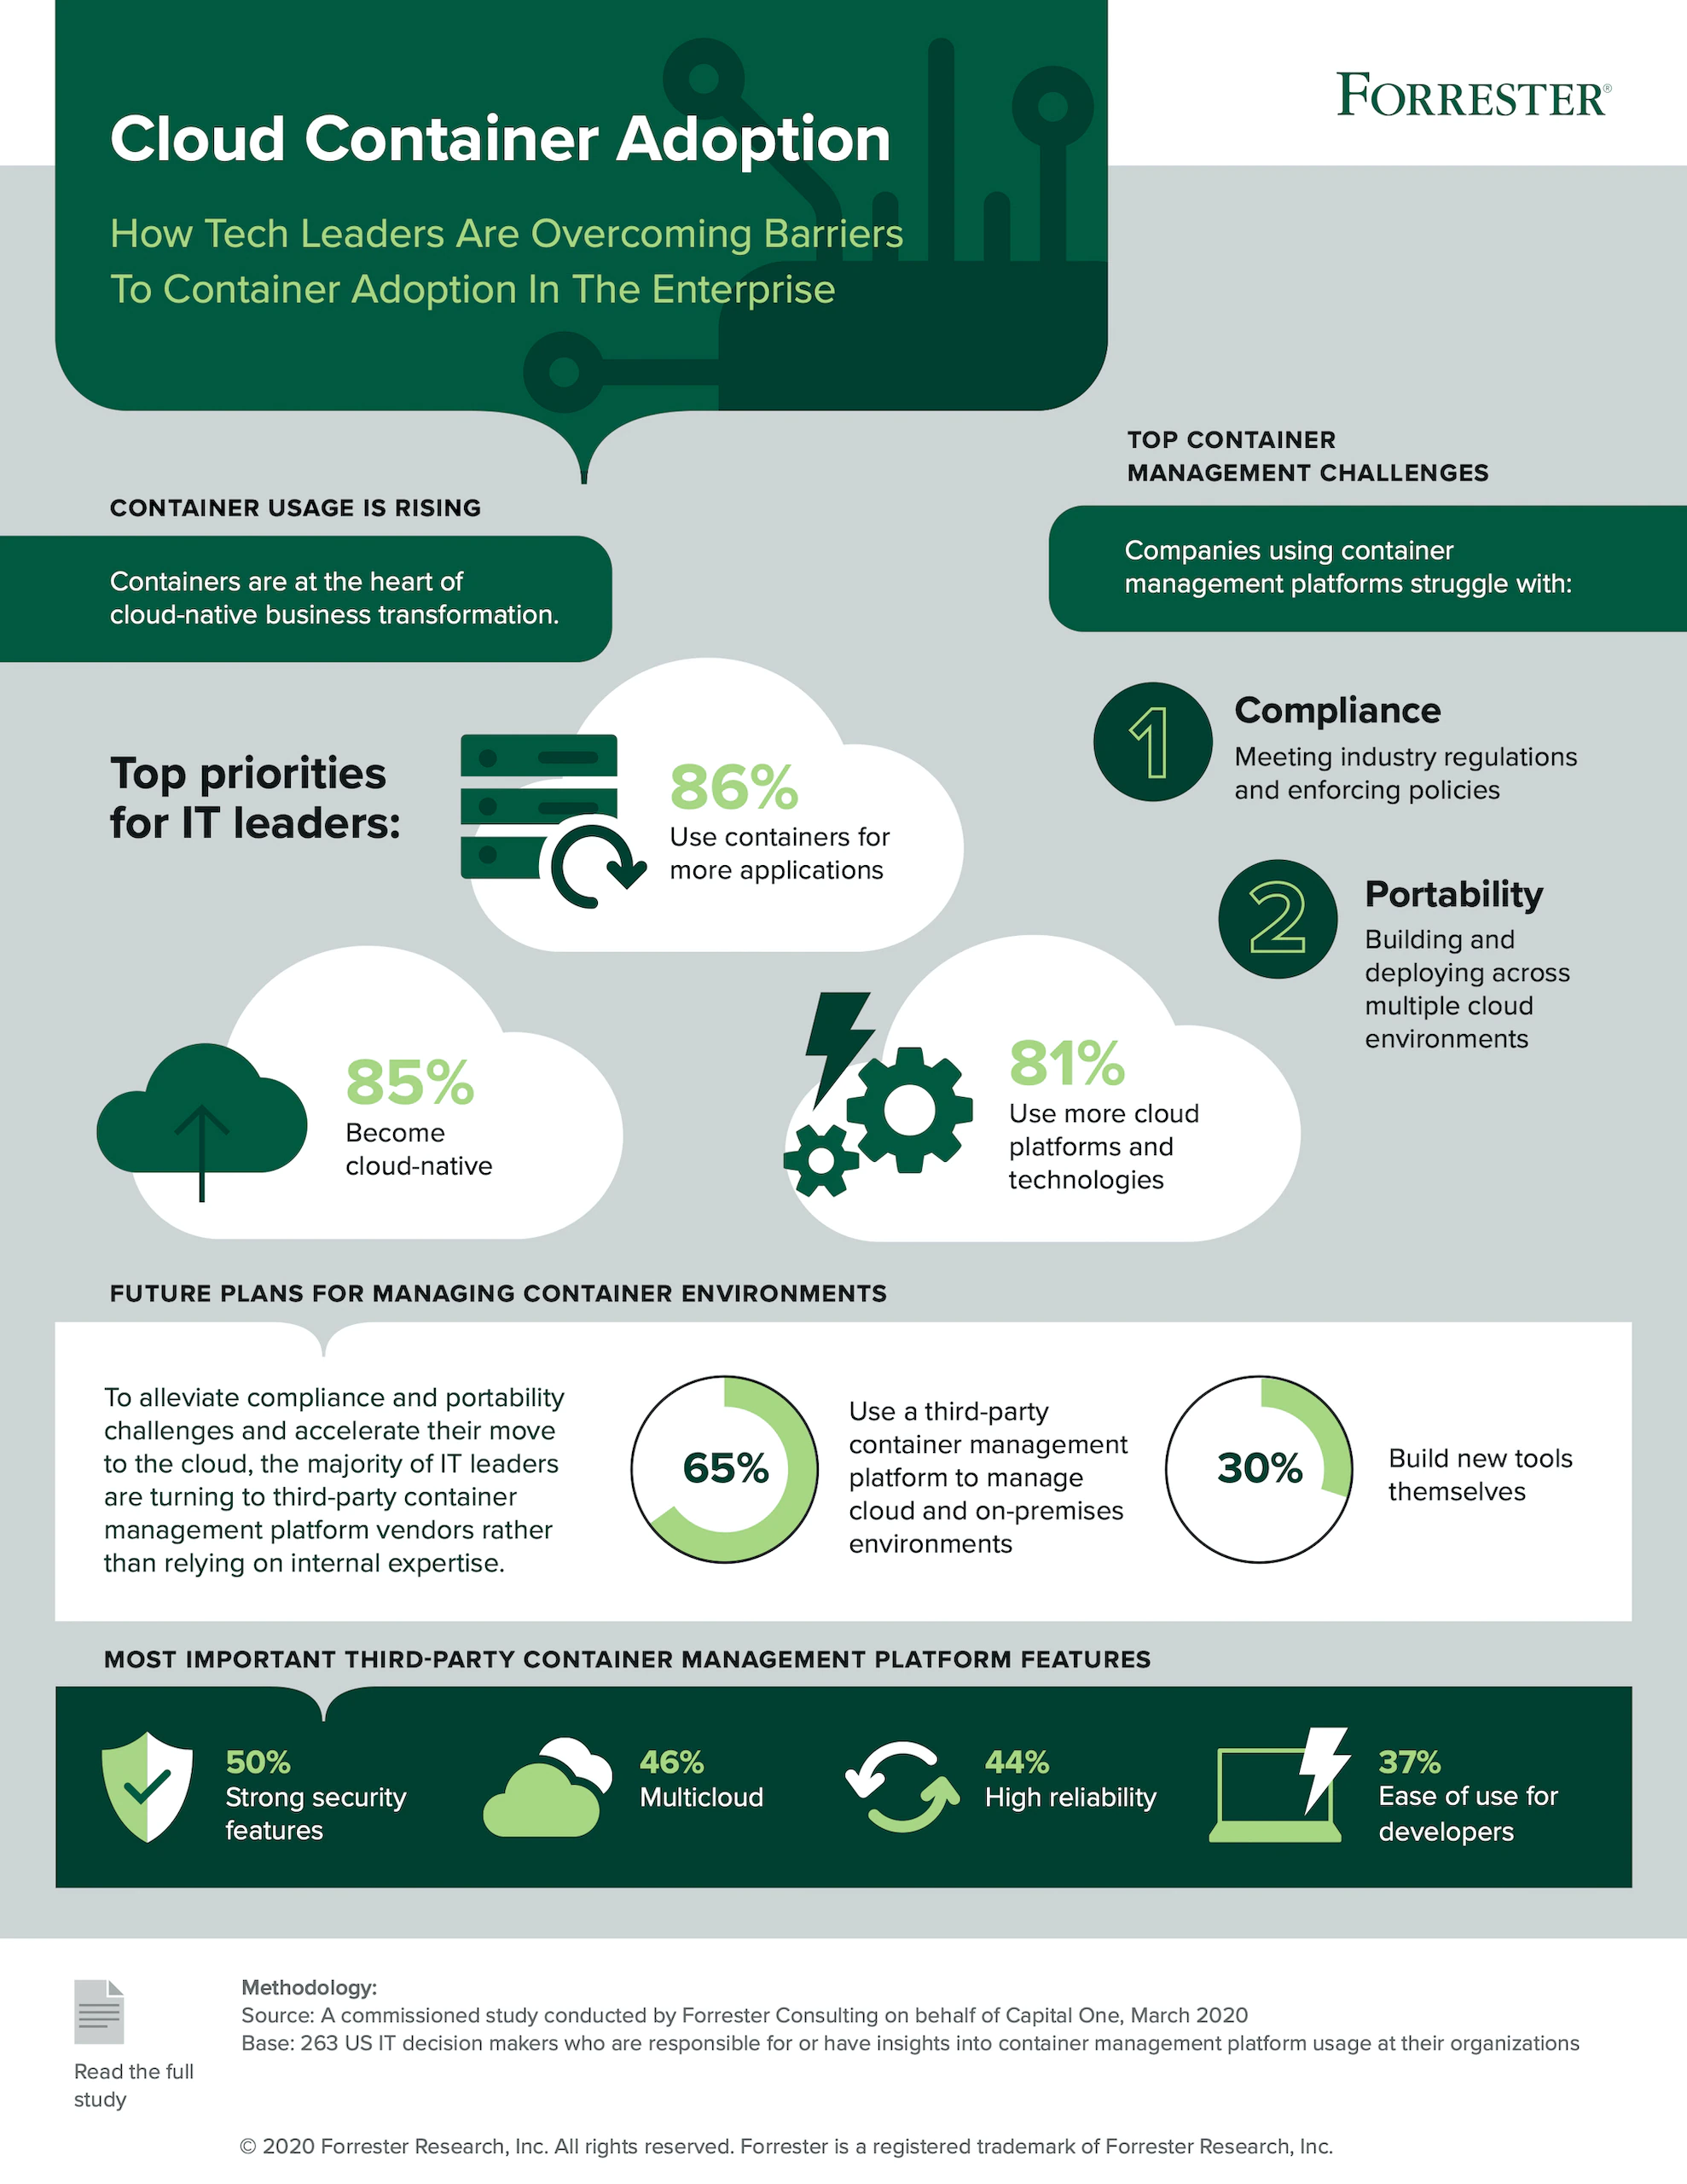
\includegraphics[width=.85\linewidth]{pictures/container-adoption-statistics-infographic.png}
    \caption{Estadísticas de adopción de tecnologías basadas en contenedores en la nube, 2020 \cite{ContainerAdoptionStatistics}.}
    \label{fig:container-stats}
\end{figure}

De entre todos los datos anteriores, es destacable el gran uso de Docker y Kubernetes
para gestionar toda esta infraestructura. En 2017, Docker representaba un 99\% de
los contenedores en uso. Sin embargo, con la compra de CoreOS por RedHat y el
lanzamiento de la OCI ha promovido el nacimiento y establecimiento de nuevas
tecnologías de contenedores que le han quitado cuota de mercado a Docker \cite{Download2018Docker2018}.
Actualmente, la distribución queda (figura \ref{fig:container-runtime}):

\begin{figure}[H]
    \centering
    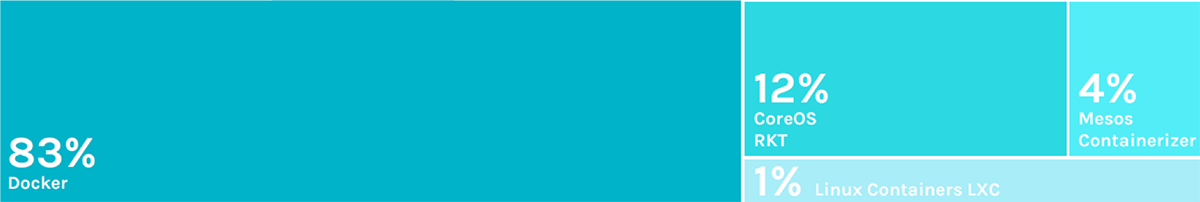
\includegraphics[width=\linewidth]{pictures/container-runtimes.png}
    \caption{Usos de tecnologías de contenedores: Docker domina, seguido por rkt y Mesos \cite{Download2018Docker2018}.}
    \label{fig:container-runtime}
\end{figure}

Todo esto nos lleva a ver que si bien aparecen alternativas nuevas Docker sigue siendo
la tecnología dominante y la que más adopción está teniendo. Esta competitividad es
muy buena ya que permite a Docker y a otras tecnologías de contenedores, como rtk de 
RedHat (CoreOS), evolucionar, seguir avanzando y mejorando. Lo interesante no es ya
usar Docker, rtk o LXC sino que se ha establecido un estándar de contenedores abierto (OCI)
y que pone las bases a lo que es una tecnología revolucionaria.